Before we begin going into two-photon processes we must first develop a few computational techniques. When dealing with a two-photon process, the transition from initial to final state is connected by an intermediate state. This intermediate state is actually a summation over all possible bound states as well as an integration over the continuum. This is computationally very intensive and difficult to deal with. Instead we will be developing a technique that uses a discrete set of variational pseudostates to represent the entire spectrum of hydrogen. As a demonstration of this technique we will be showing how the entire spectrum of hydrogen can be represented by two pseudostates for the calculation of the polarizability. The particular calculation we will be doing to represent this is a calculation of the static polarizability of hydrogen. This is a known value that can be calculated analytically and so is a strong demonstration of the power of the technique.
\section{Sturmian Basis Sets}
The dipole polarizability of an atom corresponds to the zero-frequency limit of a two-photon process. \(\Delta E\) describes the energy shift of an atom in a static electric field according to
\begin{equation}
    \Delta E = \frac{1}{2}\alpha_d F^2
\end{equation}
Where \(F\) is the field strength and $\alpha_d$ is the polarizability. In this chapter we develop computational methods for this as a test case that will be applied later to two-photon processes. The dipole polarizability is defined by the second-order perturbation expression \cite{variational}
\begin{equation}
    \alpha_{d}\equiv- E^{(2)}=-\int\sum_{n=1}^{\infty}\frac{\abs{\bra{np}eFr\cos{\theta}\ket{1s}}^{2}}{E_{n}-E_{1s}}
\end{equation}
where the summation over $n$ includes an integration over the continuous part of the spectrum, and $E^{(2)}$ is the second-order perturbation energy due to the external field.
%The hyperfine transition that is being studied is a two photon process where the jump from the ground state to the excited state is mediated by a transition to an intermediate virtual state. This is represented as a summation over all possible states and an integration over the continuum. These two photons can be any frequency so long as the sum of their energies is equal to the total transition energy\cite{loudon}. There is no conservation of energy needed with regards to the intermediate states as no real transitions are occurring\cite{loudon}

%\begin{center}

%        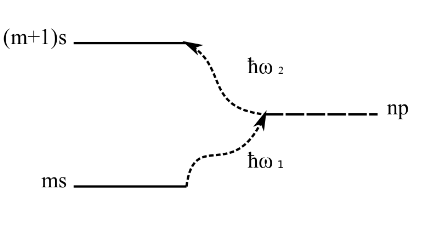
\includegraphics[width=0.4\textwidth]{images/transitioncrop.PNG}

%\end{center}
        
In this particular example the ground state is the \(1s\) state and the intermediate virtual states are represented by the p-states connected by electric dipole transitions. The expression as it stands involves a summation over the entire spectrum of p-states and then an integration over the continuum. This however is difficult to do in practice. We instead use the pseudostate method along with the variational method to sum over a discrete variational basis set with no integration over the continuum.
	The first set of using this method is generating the pseudostates. To do this we first define what sort of basis set we wish to use. Since the field-free Hamiltonian is spherically symmetric, we use spherical coordinates as this makes the resulting integrals rather elegant to evaluate analytically. Every state is expanded in the basis set of functions \(r^n e^{-\alpha r}Y_l^m(\theta,\phi)\) \cite{shark}
	\begin{equation}
    \Psi(r)=\sum_{n=1}^{N}c_{n}r^{n}e^{-\alpha r}Y_{l}^{m}(\theta,\phi)
    =\sum_n c_n \chi_n
    \end{equation}
    \begin{equation}
        \chi_n=r^n e^{-\alpha r}Y_l^m(\theta,\phi)
    \end{equation}
    where the \(c_{n}\) are linear variational parameters and \(\alpha\) is a nonlinear variational parameter. We use this particular form for our wave equations because they have the same functional form as hydrogenic wave functions. In addition, all integrals can be evaluated analytically using
    \begin{equation}
        \int_{0}^{\infty}r^{n}e^{-\alpha r}dr=\frac{n!}{\alpha^{n+1}}.
    \end{equation}
 First we must create out basis set by forming linear combinations. We do this by generating an overlap matrix whose elements are \cite{shark}.
 \begin{equation}
     \chi_{n}(r)=r^{n}e^{-\alpha r}Y_{l}^{m}(\theta,\phi)
 \end{equation}
 \begin{equation}
     O_{mn}=\bra{\chi_{m}}\ket{\chi_{n}}
 \end{equation}
  The way this matrix is orthogonalized is by the Jacobi method,(see Appendix) which works in this case because our matrix is symmetric. 

\section{Dipole Polarizability}
We now apply the sets of pseudostates to the calculation of the polarizability of ground-state hydrogen. We consider a hydrogen atom in the ground state placed in a static electric field of strength \textit{F} pointing in the \textit{z} direction. This gives rise to the perturbation \(V=eFr\cos{\theta}\). In the case of hydrogen, the first order perturbation equation can be solved analytically as further discussed below. However as a test of the pseudostate method, we will use it instead to calculate the second-order correction to the energy. This is useful because we can use this very simple example to test that the method works and can then be applied to much more complex examples. The $N$ pseudostates will be employed in the following way to calculate the second order correction to the energy.
\begin{equation}
    E^{(2)}=\sum_{n=1}^{N}\frac{\abs{\bra{n_{p}}eFr\cos{\theta}\ket{1s}}^{2}}{E_{n}-E_{1s}}
\end{equation}
Taking this with the definition of the dipole polarizability
\begin{equation}
    \alpha_{d}\equiv- E^{(2)}
\end{equation}
which for the case of the ground state of hydrogen becomes $\alpha_d=\frac{9}{2}a_{0}^{3}$ where $a_0$ is the Bohr radius. There are several things worth mentioning about this technique. The first concerns the variational parameter \(\alpha\). If we were to take our expression evaluated with a small basis set and plot is as a function of \(\alpha\) we can see that there is a rather significant variation as shown in Fig.\ref{fig:Dipole Polarizability}. However we can very plainly see an absolute maximum located at \(\alpha=1\) \cite{variational}.  We can also see that the true value of $\alpha_d$ is an upper bound to our function and no matter how large we expand our basis set that ceiling of the true value of \(4.5a_{0}^{3}\) is never exceeded. Note that all the contributions to Eq. (3.8) are positive.
\begin{figure}
    \centering
    \caption{Variational calculation of the dipole polarizability of 1s hydrogen with a two-term basis set}
    \label{fig:Dipole Polarizability}
\begin{tikzpicture}
\begin{axis}[
width=13cm,
height=10cm,
xlabel = Variational Parameter $\alpha$,
xmax = 1.4,
xmin = 0.45,
ylabel = Dipole Polarizability,
ymax = 4.5,
ymin = 4
]
\addplot[
color = black,
mark = none] table {Polar.txt};
\end{axis}
\end{tikzpicture}
\end{figure}

\begin{figure}
    \centering
    \caption{Stability of the polarizability with size of basis set}
    \label{fig:Dipole Polarizability MAXPOW}
\begin{tikzpicture}
\begin{axis}[
width=12cm,
height=10cm,
xlabel = Variational Parameter $\alpha$,
xmax = 2,
xmin = 0,
ylabel = Dipole Polarizability,
ymax = 4.55,
ymin = 0,
legend entries={$N=2$,$N=3$,$N=4$, $N=5$},
legend style={
cells={anchor=east},
legend pos=outer north east,
}
]
\addplot[
color = black,
mark = none] table {MAXPOW2.txt};
\addplot[
color = green,
mark = none] table {MAXPOW3.txt};
\addplot[
color = red,
mark = none] table {MAXPOW4.txt};
\addplot[
color = orange,
mark = none] table {MAXPOW5.txt};
\end{axis}
\end{tikzpicture}
\end{figure}
The one important thing that does change as $N$ increases is that the expression for $\alpha_d$ becomes less sensitive to the actual value of $\alpha$ used, as long as it is not too far from the optimum value $\alpha=1$. What this means is that, the larger the basis set, the less sensitively the calculated value for $\alpha_d$ depends on $\alpha$ as seen in Fig.\ref{fig:Dipole Polarizability MAXPOW}. When this method is applied to more complicated systems such as helium we can simply expand the basis set size and look for an extremum with respect to \(\alpha\). The main drawback is that the larger the basis set used, the longer the computation time. Instead a much more economical technique to look for a maximum for $\alpha_d$ as a function of $\alpha$. We can vary \(\alpha\) to find this maximum to arrive at the optimum result. When working with more complicated systems it is far more economical to use these variational parameters to find a maximum then it is to calculate using a larger basis set.

For our purposes however we can arrive at the exact result of \(4.5a_{0}^{3}\) using only a two dimensional basis set with matrix elements and energies of \cite{variational}
\begin{equation}
\begin{split}
    \psi_1&=re^{-r}-\sqrt{\frac{8}{45}}r^2 e^{-r}\\
    E_1&=-\frac{1}{10}\quad \rm{a.u.}\\
    \psi_2&=\sqrt{8} re^{-r}-2\frac{\sqrt{2}}{3}r^2 e^{-r}\\
    E_2&=\frac{1}{2}\quad \rm{a.u.}\\
\end{split}
\end{equation}
These were calculated using the Sturmian Basis set method as described in the previous section. This is extremely powerful as we are representing the entire spectrum of hydrogen with only two pseudostates.